% !TeX root = 弹性力学笔记.tex
% 第一章：平面问题的基本理论（对应 Typst 版正文）
% ------------------------------------------------------------

\section{平面应力问题与平面应变问题}

严格来说任何一个弹性力学问题都是空间问题。但是，如果所考察的弹性体具有某种特殊的形状，并且承受的是某种特殊的外力和约束，就可以把空间问题简化为近似的平面问题。

\subsection{平面应力问题}

\begin{definition}
	当分析对象是很薄的等厚度薄板（如图~\ref{fig:planestress} 所示），且只在板边上受有平行于板面并且不沿厚度变化的面力或约束，同时，体力也平行于板面并且不沿厚度变化，这时的弹性力学问题可以看作一个平面应力问题。
\end{definition}

\begin{figure}[htbp]
	\centering
	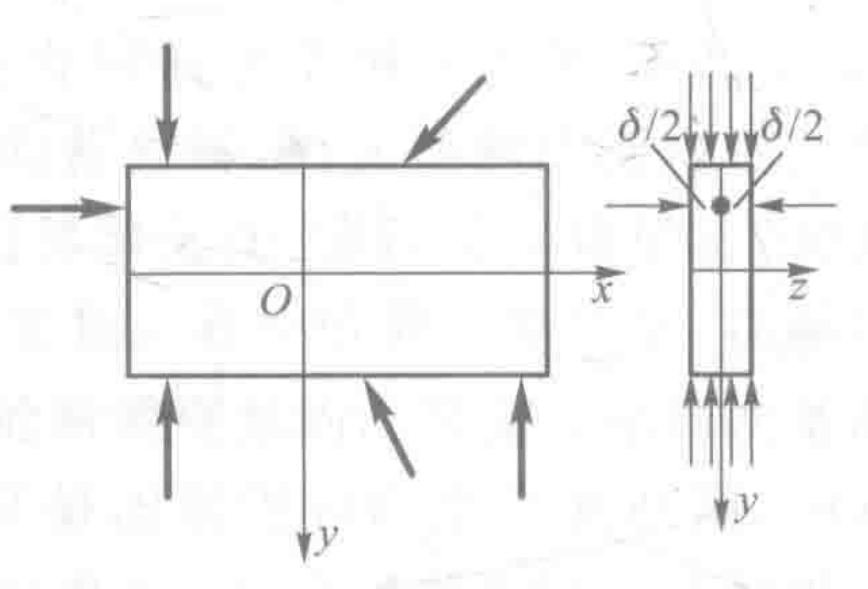
\includegraphics[width=0.5\linewidth]{figure/平面应力问题.png}
	\caption{平面应力问题}
	\label{fig:planestress}
\end{figure}

设薄板的厚度为 $\delta$，以薄板的中面为 $xy$ 面，以垂直于中面的任一直线为 $z$ 轴，因为板的前后面，即 $z=\pm\frac{\delta}{2}$ 处不受力。所以有

\[
	(\sigma_z)_{z=\pm\frac{\delta}{2}}=0 \quad
	(\tau_{zx})_{z=\pm\frac{\delta}{2}}=0 \quad
	(\tau_{zy})_{z=\pm\frac{\delta}{2}}=0
\]

因为板很薄，外力又不沿厚度变化，且应力是连续分布的，所以，可以认为在整个薄板的所有各点都有

\[
	\sigma_z=0 \quad \tau_{zx}=0 \quad \tau_{zy}=0
\]

再由切应力互等定理，于是只剩下了平行于 $xy$ 面的三个应力分量 $\sigma_x, \sigma_y, \tau_{xy}=\tau_{yx}$。同时，也因为板很薄，这三个应力分量，以及分析问题时需要考虑的应变分量和位移分量，都可以认为是不沿厚度变化的。这就是说，它们只是 $x$ 和 $y$ 的函数，不随 $z$ 而变化。

\subsection{平面应变问题}

\begin{definition}
	设有一很长的柱形体，其横截面不沿长度变化，在柱面上受有平行于横截面并且不沿长度变化的面力或约束，同时体力也平行于横截面并且不沿长度变化（如图~\ref{fig:planestrain} 所示），这时的弹性力学问题可以看作一个平面应变问题。
\end{definition}

工程中沿长度方向很长的挡土墙、隧道、管道、重力坝等，除去靠近两端的一小段外，中间部分都可近似按平面应变问题处理。

\begin{figure}[htbp]
	\centering
	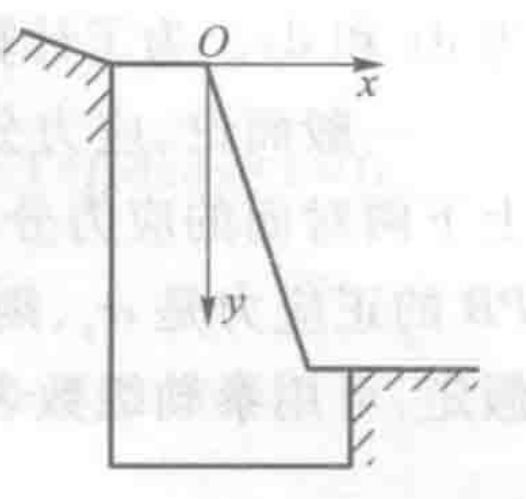
\includegraphics[width=0.5\linewidth]{figure/平面应变问题.png}
	\caption{平面应变问题}
	\label{fig:planestrain}
\end{figure}

假想柱形体的长度趋于无限，以任一横截面为 $xy$ 面，任一纵线为 $z$ 轴。由于截面形状和所受外力都不沿 $z$ 方向变化，所以一切应力分量、应变分量和位移分量都只是 $x$ 和 $y$ 的函数，不随 $z$ 变化。此外，柱体既然无限长，任一横截面都可以看作对称面，截面内的各点只可能沿 $x$、$y$ 方向移动，不可能沿 $z$ 方向移动（否则对称面两侧的材料将发生相对错动）。于是

\[
	u=u(x,y), \qquad v=v(x,y), \qquad w=0
\]

代入几何方程，得到

\[
	\varepsilon_z=\frac{\partial w}{\partial z}=0, \qquad
	\gamma_{zx}=\frac{\partial w}{\partial x}+\frac{\partial u}{\partial z}=0, \qquad
	\gamma_{zy}=\frac{\partial w}{\partial y}+\frac{\partial v}{\partial z}=0
\]

这就是说，纵向正应变 $\varepsilon_z$ 和两个纵向切应变 $\gamma_{zx}$、$\gamma_{zy}$ 都等于零，只剩下平行于 $xy$ 面的三个应变分量 $\varepsilon_x$、$\varepsilon_y$、$\gamma_{xy}$，这正是「平面应变」这一名称的由来。

应变分量是三个，应力分量却不只三个。设材料的弹性模量为 $E$，泊松比为 $\mu$，切变模量为 $G=\frac{E}{2(1+\mu)}$，由物理方程（广义胡克定律）

\[
	\left.
	\begin{aligned}
		\varepsilon_x & = \frac{1}{E}\left[\sigma_x-\mu\left(\sigma_y+\sigma_z\right)\right] \\
		\varepsilon_y & = \frac{1}{E}\left[\sigma_y-\mu\left(\sigma_z+\sigma_x\right)\right] \\
		\varepsilon_z & = \frac{1}{E}\left[\sigma_z-\mu\left(\sigma_x+\sigma_y\right)\right] = 0 \\
		\gamma_{xy} & = \frac{2(1+\mu)}{E}\tau_{xy}
	\end{aligned}
	\right\}
\]

其中最后一个关于 $\varepsilon_z$ 的式子给出了 $\sigma_z$ 与 $\sigma_x$、$\sigma_y$ 的关系，即

\[
	\sigma_z=\mu\left(\sigma_x+\sigma_y\right)
\]

可见平面应变问题中虽无 $z$ 方向的应变，却有 $z$ 方向的应力；它一般不等于零，只是不独立，可以由 $\sigma_x$、$\sigma_y$ 直接算出。把上式代回前两式，得到

\[
	\varepsilon_x=\frac{1-\mu^{2}}{E}\left(\sigma_x-\frac{\mu}{1-\mu}\sigma_y\right), \qquad
	\varepsilon_y=\frac{1-\mu^{2}}{E}\left(\sigma_y-\frac{\mu}{1-\mu}\sigma_x\right), \qquad
	\gamma_{xy}=\frac{2(1+\mu)}{E}\tau_{xy}
\]

把平面应力问题的物理方程

\[
	\varepsilon_x=\frac{1}{E}\left(\sigma_x-\mu\sigma_y\right), \qquad
	\varepsilon_y=\frac{1}{E}\left(\sigma_y-\mu\sigma_x\right), \qquad
	\gamma_{xy}=\frac{2(1+\mu)}{E}\tau_{xy}
\]

与上式逐项对照，可以看出：只要把 $E$ 换成 $\frac{E}{1-\mu^{2}}$，把 $\mu$ 换成 $\frac{\mu}{1-\mu}$，平面应力问题的物理方程就变成了平面应变问题的物理方程。因此两类平面问题在数学形式上是完全相同的：独立未知量都是 $\sigma_x$、$\sigma_y$、$\tau_{xy}$、$\varepsilon_x$、$\varepsilon_y$、$\gamma_{xy}$、$u$、$v$ 共 8 个，方程也都是 2 个平衡微分方程、3 个几何方程、3 个物理方程，共 8 个，而且边界条件的形式也相同。

\begin{keybox}[小结]
	平面应力问题与平面应变问题的控制方程和边界条件形式一致，只是物理方程中的弹性常数不同。因此以后导出的公式和解答，凡含有 $E$、$\mu$ 的，都不必重新推导：由平面应力问题的结果按
	\[
		E\rightarrow\frac{E}{1-\mu^{2}}, \qquad \mu\rightarrow\frac{\mu}{1-\mu}
	\]
	替换，即得平面应变问题的结果；反之，作相反的替换即可。
\end{keybox}

\begin{note}
	两类问题的区别在于形状与受力的组合，而不在于问题是否「二维」。薄板受板面内的力是平面应力问题，此时 $\sigma_z=0$ 而 $\varepsilon_z\neq0$（板厚可以自由改变）；长柱体受横截面内的力是平面应变问题，此时 $\varepsilon_z=0$ 而 $\sigma_z\neq0$。后者容易被误认为「z 方向没有应力」，实际 $\sigma_z=\mu(\sigma_x+\sigma_y)$ 往往不可忽略，在混凝土坝、隧洞衬砌等按平面应变计算的构件中，仍需用它校核纵向强度。
\end{note}

